\chapter{Introduction}
\label{chap:intro}

\begin{figure}
\caption{The Internet's four-layer model}
\label{f:stack}
\begin{centering}
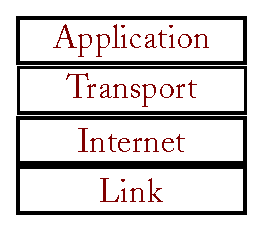
\includegraphics{layers.pdf}

\end{centering}
\end{figure}

\begin{figure}
\caption{As the Internet has evolved, researchers have created at
  least 40 mechanisms to govern resource allocation on the
  network---both entirely distributed schemes (``end-to-end'') and
  ones that include code running ``in-net.''}
\label{f:march}

\vspace{\baselineskip}

\begin{centering}
\noindent 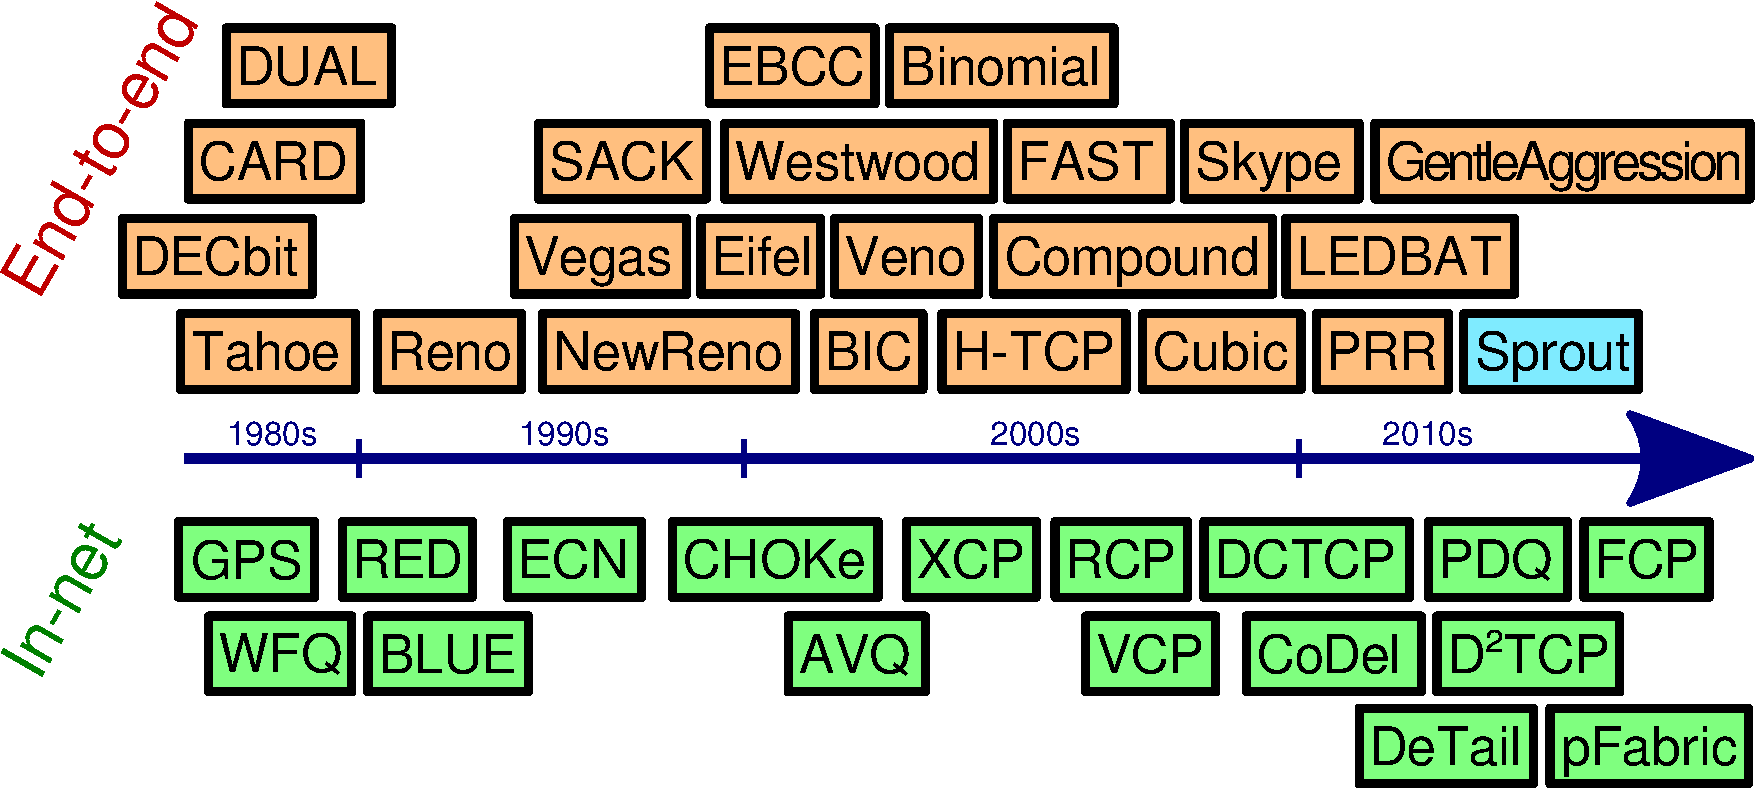
\includegraphics[width=\textwidth]{march2-all.pdf}

\end{centering}
\end{figure}

Over the last 25 years, the Internet has transformed from an academic
networking experiment into a global utility with billions of
users. As part of this transformation, every layer of the Internet
``stack'' has seen dramatic change.

At the link layer, technologies that did not exist 25 years
ago now dominate---including wireless local-area networks (Wi-Fi),
cellular networks, datacenter interconnects, and transoceanic links
with high delay.

One layer up, at the Internet layer, mobility is now
ubiquitous. User devices regularly change their interface IP addresses
as they roam from network to network.

At the top layer of the Internet stack---the application
layer---none of the dominant applications of today existed 25 years
ago, including the World Wide Web and its short-length flows,
progressive-download video applications (e.g., YouTube and Netflix),
and real-time streaming video (e.g., Skype and Facetime).

All of the Internet has had to grapple with this continuous
evolution. How should the protocols of the transport layer,
sitting in the middle of the stack between the application and the
Internet, adapt to changing applications above them and
evolving networks below?

One legitimate answer may be that transport-layer protocols need not
adapt. If the network or applications evolve, and a transport
protocol no longer works adequately alongside then, we can simply stop
using the protocol and design a fresh one that matches the new
circumstances.

This approach broadly characterizes the Internet's extraordinarily
successful path over the last 25 years. Looking at just one
function of the transport layer---congestion control, the job of
dividing up the network's resources among contending
users---researchers have accommodated new applications and network
behaviors by devoting considerable effort to develop new
mechanisms, at least 40 in total so far (Figure \ref{f:march}).

Despite its success, this approach imposes costs. In defining
transport-layer protocols by their \emph{mechanisms}---by the actual
behavior of endpoints that execute the protocol---we leave implicit
the assumptions that the mechanism makes about the behavior of other
layers and the policy that the mechanism is built to pursue.

For contemporary protocols (e.g., TCP Cubic, the current default in
Linux), it's challenging to state the assumptions that the transport
makes about lower layers and to predict when those assumptions will no
longer hold. This presents a difficulty for link-layer designers who
wish to create new networking technologies. Because of Cubic's
prevalence, it has become a \emph{de facto} requirement that Cubic
perform well over any network. To achieve adequate performance, the
designer of the new link layer must make sure to satisfy Cubic's
implicit assumptions.

This has led to the ``bufferbloat''\cite{bufferbloat} problem:
believing that the transport layer will interpret losses as a signal
to slow down, the network tries to drop packets as rarely as
possible. It has also led to a lack of parallelism in Internet
routing---flows only take one path, even if striping across
multiple paths could yield a speedup---on the grounds that the
transport protocol might interpret out-of-order packets as a
pathology.

On the flip side, it is not easy to adjust the transport
layer's assumptions in order to accommodate a new kind of
network. There's no way to tweak the requirements and then retrace the
same design process that the protocol's designers followed, to find the
mechanism they would have produced given a different starting point.

%\section{Showing our work in protocol design}

This thesis proposes that the transport layer should adapt
programmatically to whatever the layers below may do, and whatever the
application above it wants. Protocol designers should specify the
\emph{policy}---namely, what assumptions they want to make about the
network and what kind of performance the application is interested
in---and let computers worry about translating this into the mechanism
of congestion control.

By ``showing our work'' clearly enough for a computer to create the
design, tweaking a protocol's assumptions becomes a matter of changing
the inputs to a computer program and running it again. My colleagues
and I have found that this approach yields better peformance than
conventional protocols, while allowing adjacent layers to evolve more
freely. It's not clear when computer-generated protocols will be
practically deployed on the broad Internet, but what computers can
teach us about protocol design can be applied to help humans create
better protocols now.

\section{Summary of results}

My colleagues and I have built two systems that explore the benefits
of automated, objective-driven congestion-control protocol design.

\textbf{Sprout} (Chapter~\ref{chap:sprout}) is a transport protocol
designed to carry high-throughput interactive traffic, such as a
videoconference, over a cellular network. Sprout includes an explicit
model of the dynamics of cellular networks and makes predictions about
future performance by inferring a distribution over the current state
of the network and evolving the model forward. Its control
strategy---how much data to send at a given moment---is a function of
those predictions and of an explicit objective: maximize throughput,
but cap in-network delays to be at most 100~ms with high
probability.

In a trace-driven experimental evaluation (details in
\S\ref{sprout:eval}), Sprout gave 2-to-4 times the throughput and
7-to-9 times less delay than Skype, Apple Facetime, and Google
Hangouts:

\begin{center}
\noindent \begin{tabular}{|l|c|c|}
\hline
Sprout vs. & Avg.~speedup & Delay reduction \\
\hline
\hline
Skype & $2.2\times$ & $7.9\times$\\
Hangout & $4.4\times$ & $7.2\times$\\
Facetime & $1.9\times$ & $8.7\times$\\
\hline
Compound & $1.3\times$ & $4.8\times$\\
TCP Vegas & $1.1\times$ & $2.1\times$\\
LEDBAT & no change & $2.8\times$\\
Cubic & \cellcolor{red!20}$0.91\times$ & $79\times$\\
%\hline
%Cubic-CoDel & \cellcolor{red!20}$0.70\times$ & $1.6\times$ (0.50~s) \\
%CUBIC/CoDel & & \\
%Compound/CoDel & & \\
\hline
\end{tabular}

{\footnotesize Adapted from Figure~\ref{f:sproutcompe2e}.}

\end{center}

\textbf{Remy} (Chapter~\ref{chap:remy}) generalizes Sprout to address
the classical problem of \emph{multi-agent} congestion control, where
independent users contend for the same limited network resource. Remy
is a protocol-design tool that takes, as input, a set of assumptions
about the uncertain network and workload, and an objective to pursue
on behalf of the application.

On a simulated 15~Mbps link with eight senders contending and an RTT
of 150~ms, a computer-generated congestion-control algorithm achieved
the following improvements in median throughput and reductions in
median queueing delay over these existing protocols:

\begin{center}

\begin{tabular}{|l|c|c|}
\hline
Protocol & Median speedup & Median delay reduction \\
\hline
\hline
Compound & $2.1\times$ & $2.7\times$ \\
NewReno & $2.6\times$ & $2.2\times$ \\
Cubic & $1.7\times$ & $3.4\times$ \\
Vegas & $3.1\times$ & $1.2\times$ \\
\hline
Cubic/sfqCoDel & $1.4\times$ & $7.8\times$ \\
XCP & $1.4\times$ & $4.3\times$ \\
\hline
\end{tabular}

{\footnotesize Adapted from \S\ref{sec:remyresults}.}

\end{center}

\section{What computers can teach us about congestion control}

We can learn about transport-protocol design by observing what makes
automated protocol-design tools successful. By looking at \emph{what
  information} turned out to be valuable to Sprout and Remy, and
\emph{what behaviors} characterize the successful computer-generated
algorithms, we have been able to develop an intuition as to what
successful new designs might look like and why Sprout and Remy are
able to outperform current protocols.

\subsection{Algorithms should collect rate estimates as signals}

Today's congestion-control protocols generally pay attention to a
small number of signals derived from packets arriving at the receiver,
or acknowledgments arriving back at the sender. Classical TCP schemes,
such as NewReno~\cite{newreno} and Cubic~\cite{cubic}, attempt to
detect packet loss as a proxy for in-network buffer
overflow. Delay-based schemes such as Vegas~\cite{vegas} detect
increasing round-trip delay, as a proxy for growing standing queues
inside the network.

Researchers and practitioners have proposed that the network should
provide additional information helpful for inferring the presence of
congestion~\cite{ecn,xcp,rcp}, but these schemes have not been widely
deployed.

Sprout and Remy have found that more useful information is available
from the data already provided by today's networks. In particular,
estimates of the rates of packet transmission and reception proved to
be crucial to helping these systems outperform existing algorithms.

\begin{figure}
\caption{Sprout measures the \textbf{rate} of packet arrivals at the
  receiver, forecasts the time required to drain the current queue,
  and tries to steer this quantity not to exceed a tenth of a
  second. Based on this technique, Sprout achieves less end-to-end
  delay than the other algorithms, while achieving almost as much
  throughput as TCP Cubic. From Figure~\ref{f:allgraphs} (Verizon LTE
  Downlink).}

\vspace{\baselineskip}

\def\svgwidth{\textwidth}\footnotesize\import{dotgraphs3/}{VerizonLTE-Downlink-minus1.pdf_tex}
\end{figure}

